\subsection{Camera Usability}
\label{sec:camera-usability}
\label{sec:draft-background}

The Samsung Galaxy camera must provide high-quality final images and a responsive capture experience.
To improve final image quality, the camera performs post-processing tailored to the camera mode and scene conditions.
This processing typically includes multi-frame composition, which combines complementary information from multiple frames captured for a single shutter input.
For capture responsiveness, the draft sequence provides users with prompt visual feedback before post-processing completes, and parallel capture substantially shortens the shot-to-shot interval by allowing capture requests to overlap.

\myparagraph{Draft sequence}
The draft sequence comprises the processing stages that produce the draft image, which is later replaced by the final image.
The draft image was originally generated from a single captured frame without multi-frame composition.
The draft and final images could therefore differ in appearance, making the replacement noticeable to users.
These differences were particularly pronounced for captures with the Filter or Watermark option enabled, because these effects were applied only to the final image.
To apply these effects to the draft image as well, Samsung added the corresponding single-frame stages to the draft sequence.

% Notes: docs/exhibits.md#fig_draft_final_gap
\begin{figure}[!ht]
  \centering
  \setlength{\tabcolsep}{1pt}%
  % All views are the same 1:1 frame (1080 bp source);
  % the zoom box keeps the source region x 162--702, y 695--875 bp from the bottom.
  % TODO: Replace the middle panel and its crop with the actual draft image
  % produced by lightweight multi-frame composition. Both temporarily reuse
  % fig_draft_final_gap_final.jpg; the caption explicitly marks this placeholder.
  \begin{tabular}{@{}ccc@{}}
    \begin{tikzpicture}
      \node[inner sep=0, anchor=south west] (im) at (0,0)
        {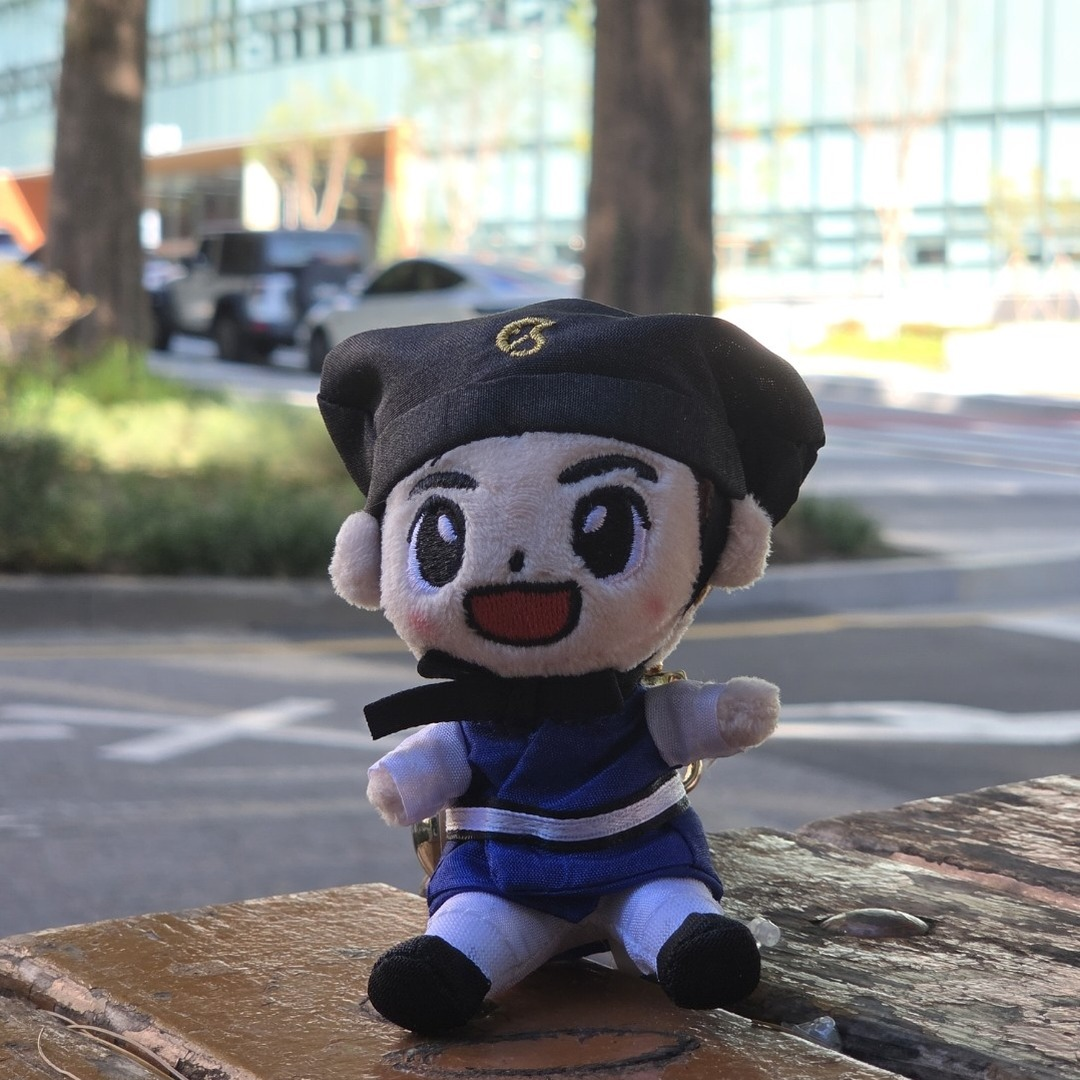
\includegraphics[width=0.325\columnwidth]{figures/fig_draft_final_gap_draft.jpg}};
      \begin{scope}[x={(im.south east)}, y={(im.north west)}]
        \draw[orange, line width=0.8pt] (0.15,0.6435) rectangle (0.65,0.8102);
      \end{scope}
    \end{tikzpicture} &
    \begin{tikzpicture}
      \node[inner sep=0, anchor=south west] (im) at (0,0)
        {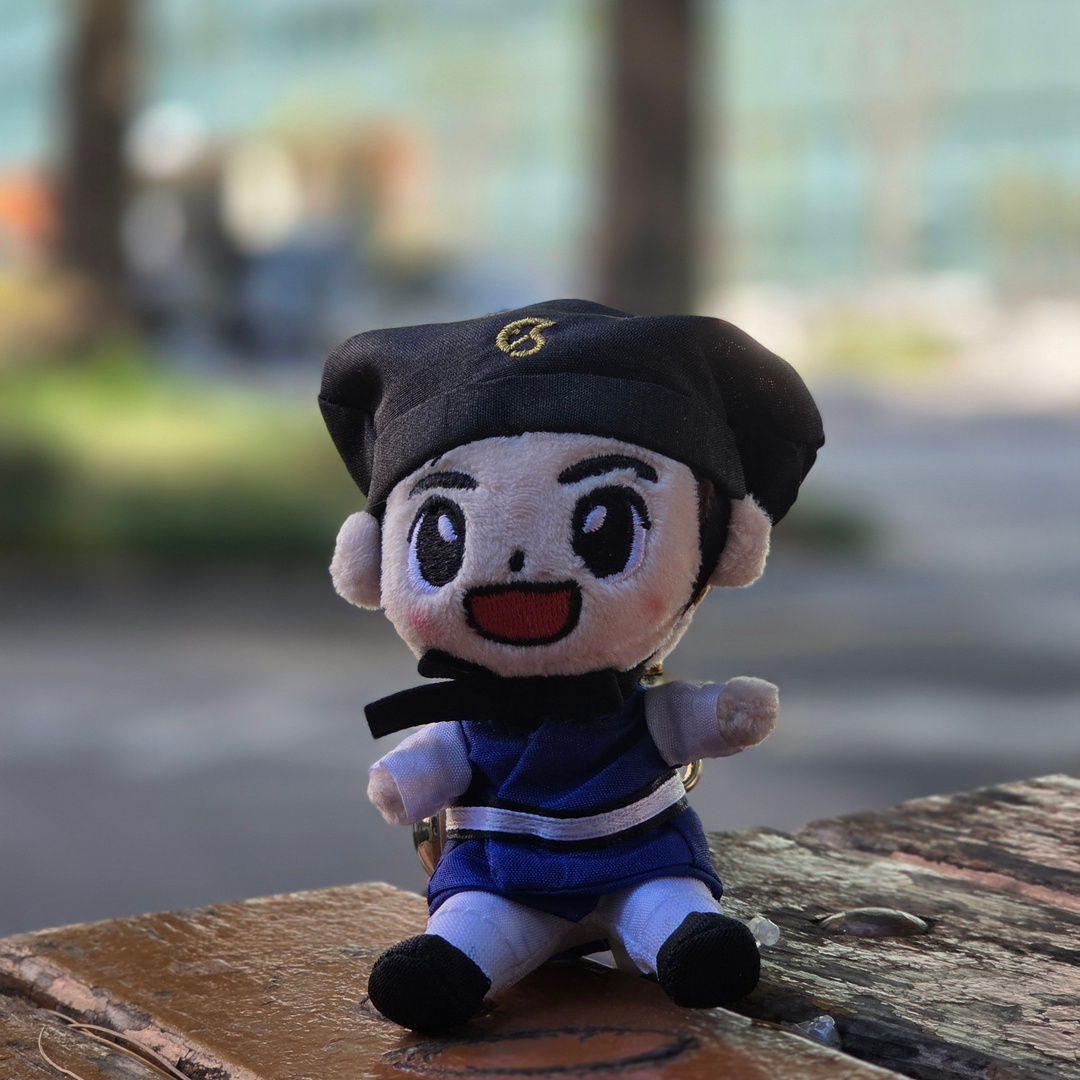
\includegraphics[width=0.325\columnwidth]{figures/fig_draft_final_gap_final.jpg}};
      \begin{scope}[x={(im.south east)}, y={(im.north west)}]
        \draw[orange, line width=0.8pt] (0.15,0.6435) rectangle (0.65,0.8102);
      \end{scope}
    \end{tikzpicture} &
    \begin{tikzpicture}
      \node[inner sep=0, anchor=south west] (im) at (0,0)
        {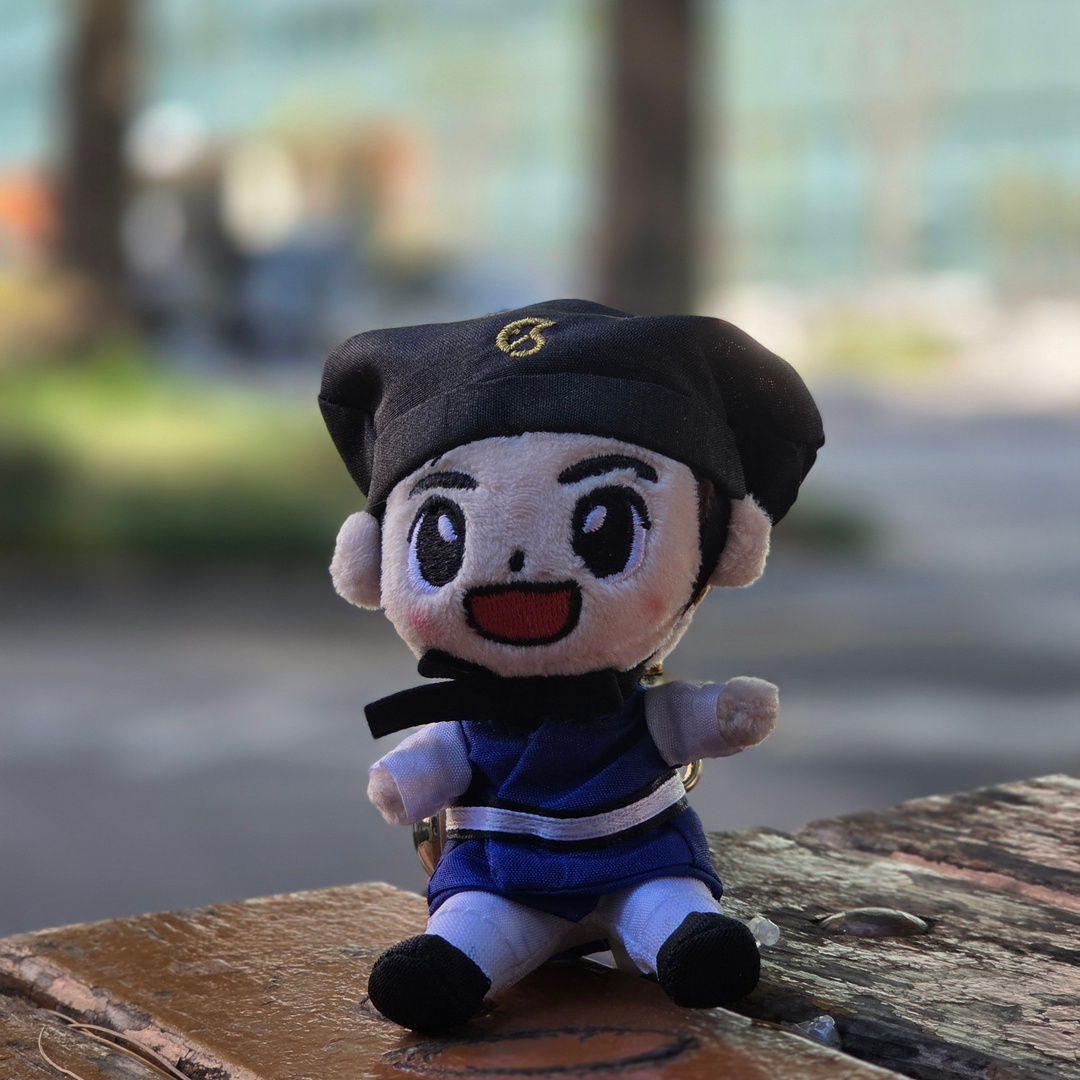
\includegraphics[width=0.325\columnwidth]{figures/fig_draft_final_gap_final.jpg}};
      \begin{scope}[x={(im.south east)}, y={(im.north west)}]
        \draw[orange, line width=0.8pt] (0.15,0.6435) rectangle (0.65,0.8102);
      \end{scope}
    \end{tikzpicture} \tabularnewline[1pt]
    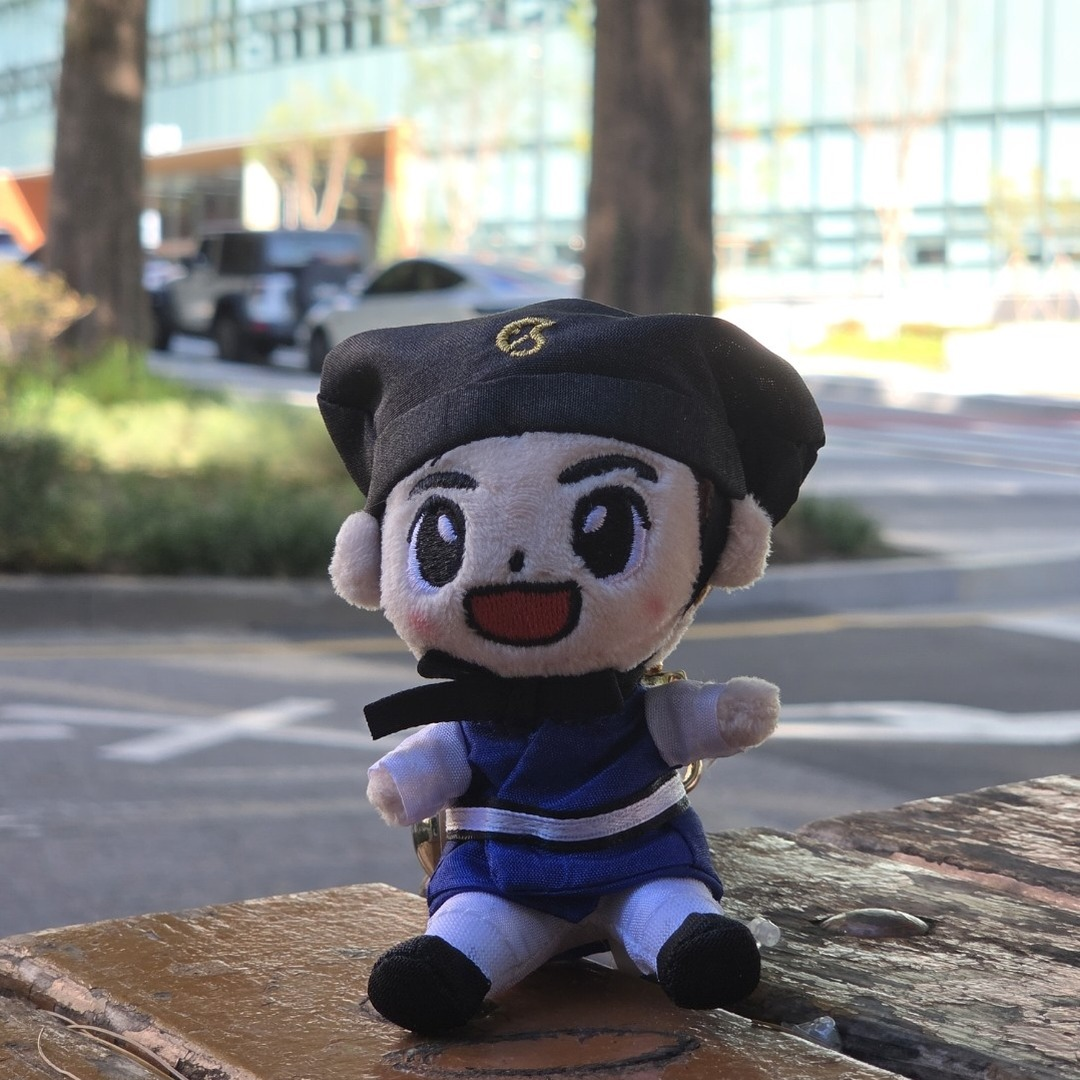
\includegraphics[width=0.325\columnwidth, trim=162 695 378 205, clip]{figures/fig_draft_final_gap_draft.jpg} &
    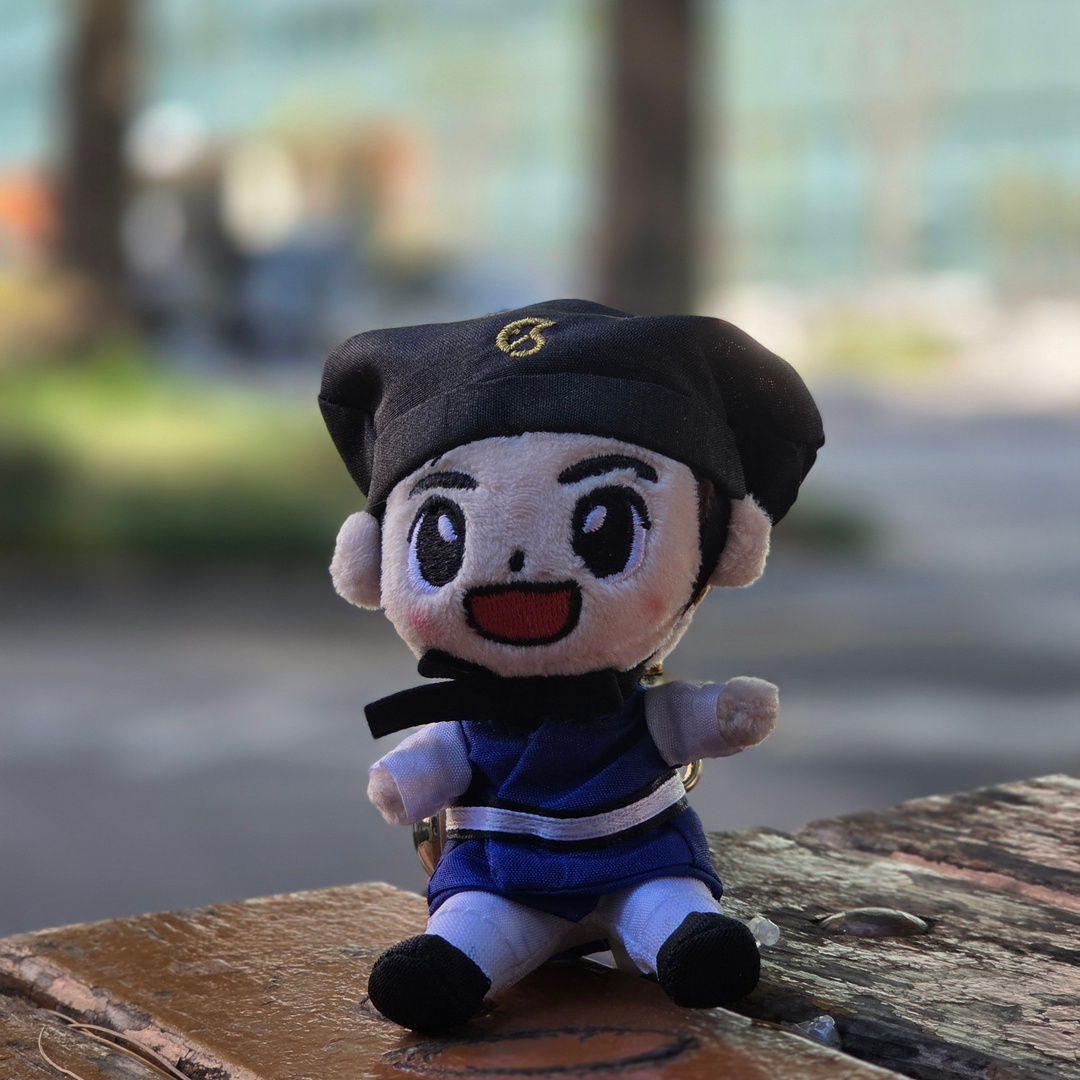
\includegraphics[width=0.325\columnwidth, trim=162 695 378 205, clip]{figures/fig_draft_final_gap_final.jpg} &
    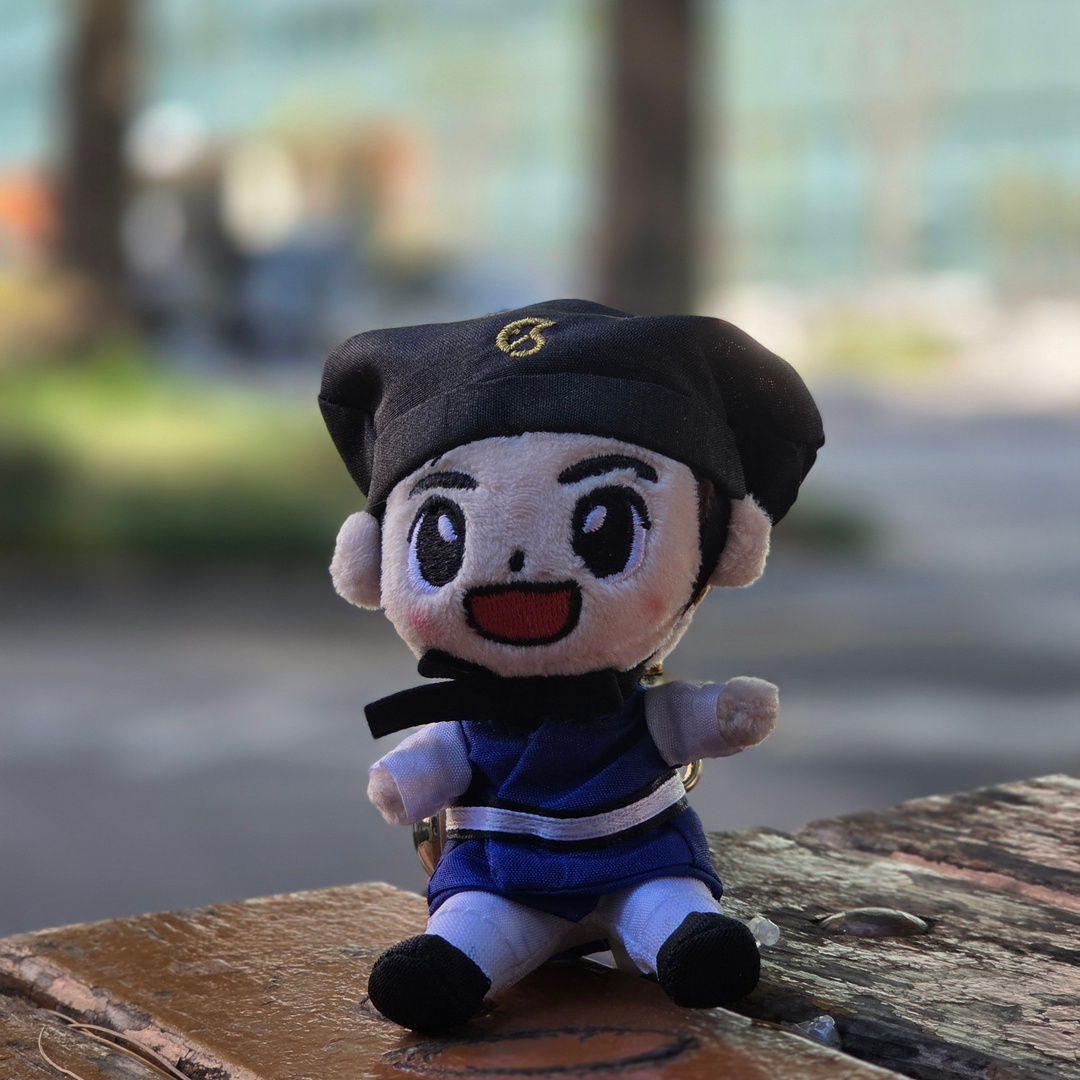
\includegraphics[width=0.325\columnwidth, trim=162 695 378 205, clip]{figures/fig_draft_final_gap_final.jpg}
    \tabularnewline[2pt]
    \parbox[t]{0.325\columnwidth}{\centering\scriptsize (a) Draft image} &
    \makebox[0.325\columnwidth][c]{%
      \parbox[t]{0.41\columnwidth}{\centering\scriptsize
        (b) Draft image with \\lightweight multi-frame composition}} &
    \parbox[t]{0.325\columnwidth}{\centering\scriptsize (c) Final image}
  \end{tabular}
  \caption{Draft--final visual differences in Portrait mode.}
  \label{fig:draft-final-gap}
\end{figure}


As post-processing has advanced over the years and improved final image quality, the visual gap between the draft and final images has continued to widen.
Figure~\ref{fig:draft-final-gap}(a) and~(c) illustrate this gap in Portrait mode.
Post-processing also came to require more computation and resources.
To preserve foreground responsiveness, Samsung deferred the start of post-processing in certain shot modes until the camera application entered the background.
This delays the generation of the final image, so users checking a photo after capture may see the draft image for longer.
Reducing the draft--final visual gap therefore became more important.

To narrow this visual gap, Samsung extended the draft sequence to support a lightweight version of the multi-frame composition used in post-processing.
Figure~\ref{fig:draft-final-gap}(b) shows the draft image produced with lightweight multi-frame composition.
It is closer to the final image in~(c) than the original draft image in~(a), so the replacement is less noticeable.

\myparagraph{Parallel capture}
\label{sec:parallel-capture}
Parallel capture allows the camera application to accept the next shutter input before the preceding capture has produced its draft image.
The camera framework receives a capture-availability signal, \texttt{captureAvailable}, from the hardware abstraction layer (HAL) and forwards it to the application, opening the next capture opportunity.
However, draft sequences execute one at a time on a single draft worker to preserve capture order and limit peak memory demand.
Each draft sequence enters the draft queue after its input frames and metadata have been collected.
Later captures must therefore wait in the draft queue when capture requests arrive faster than the worker completes draft sequences.
